\section{Getting started}


\subsection{Additive manifacturing}
\begin{frame}{Additive manifacturing (AM)}
\begin{columns}
	\begin{column}{0.6\textwidth}
		\begin{itemize}[<+->]
			\item Traditional: subtractive (i.e. \emph{removing} material)
			\item Additive manifacturing: \emph{adding} material
			\item Layer by layer
			\begin{tikzpicture}
				\draw[white] (0,0) -- (0,0.5);
				\node (model) [flowchart, visible on=<4->] at (0,0) {3D model / CAD};
				\node (slicing) [flowchart, visible on=<5->] at (0,-1.1) {Slicing into layers};
				\node (producing) [flowchart, visible on=<6->] at (0,-2.2) {Producing \& stacking};
				\node (result) [flowchart, visible on=<7->] at (0,-3.3) {Physical 3D object};
				\draw [arrow, visible on=<5->] (model) -- (slicing);
				\draw [arrow, visible on=<6->] (slicing) -- (producing);
				\draw [arrow, visible on=<7->] (producing) -- (result);
				%\draw [brown] (current bounding box.south west) rectangle (current bounding box.north east);
			\end{tikzpicture}
		\end{itemize}
	\end{column}
	\begin{column}{0.4\textwidth}
		\visible<3->{
		\begin{figure}
			\centering
			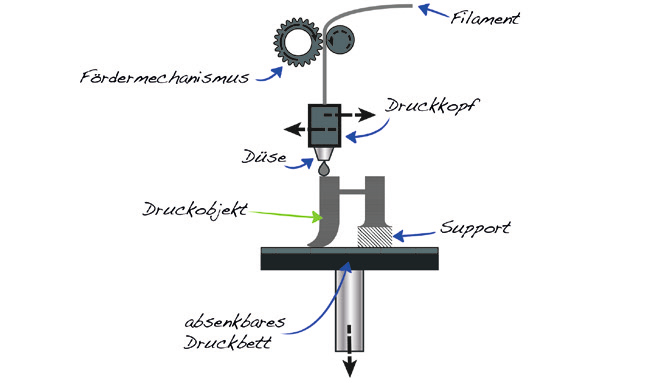
\includegraphics[trim=30 0 120 0, clip, width=\textwidth]{theory/img/fdm.png}
			\caption{AM using FDM \cite{horsch20143d}.}
		\end{figure}
		}
	\end{column}
\end{columns}
\end{frame}


\begin{frame}{Selective laser melting (SLM)}
\begin{columns}
	\begin{column}{0.5\textwidth}
		\begin{itemize}[<+->]
			\item Mostly industrial applications
			\item Material as powder
			\item Powder particles fused together by laser
			\item Popular alloys
			\begin{itemize}
				\item Titanium based (e.g. Ti6Al4V in aerospace engineering)
				\item Aluminium based (e.g. in automotive industry)
			\end{itemize}
		\end{itemize}
	\end{column}
	\begin{column}{0.5\textwidth}
		\begin{figure}
			\centering
			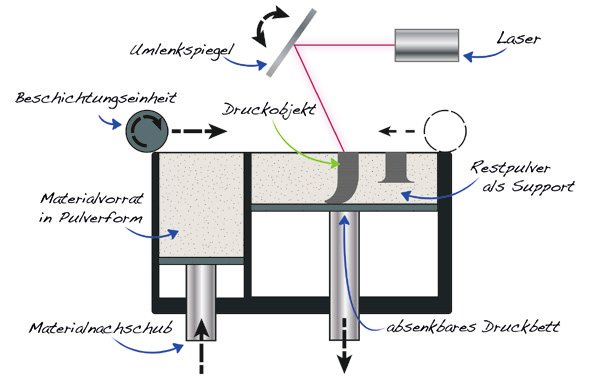
\includegraphics[width=\textwidth]{theory/img/sls_slm.png}
			\caption{AM using SLM \cite{horsch20143d}.}
		\end{figure}
	\end{column}
\end{columns}
\end{frame}


\begin{frame}{Defects in SLM - Porosities and Cracks}
\begin{columns}
	\begin{column}{0.5\textwidth}
		\visible<2->{
		\begin{figure}
			\centering
			\captionsetup{justification=centering}
			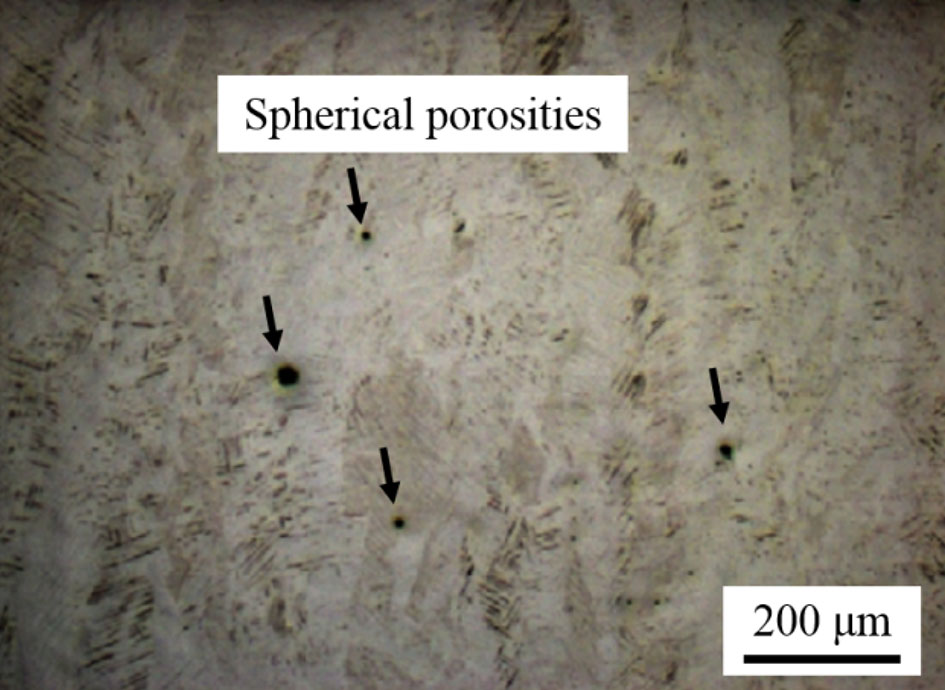
\includegraphics[width=0.9\textwidth]{theory/img/defects/porosities.png}
			\caption{Spherical porosities (enclosed gas) of different sizes \cite{zhang2017defect}}
		\end{figure}
		}
	\end{column}
	\begin{column}{0.5\textwidth}
		\visible<3->{
		\begin{figure}
			\centering
			\captionsetup{justification=centering}
			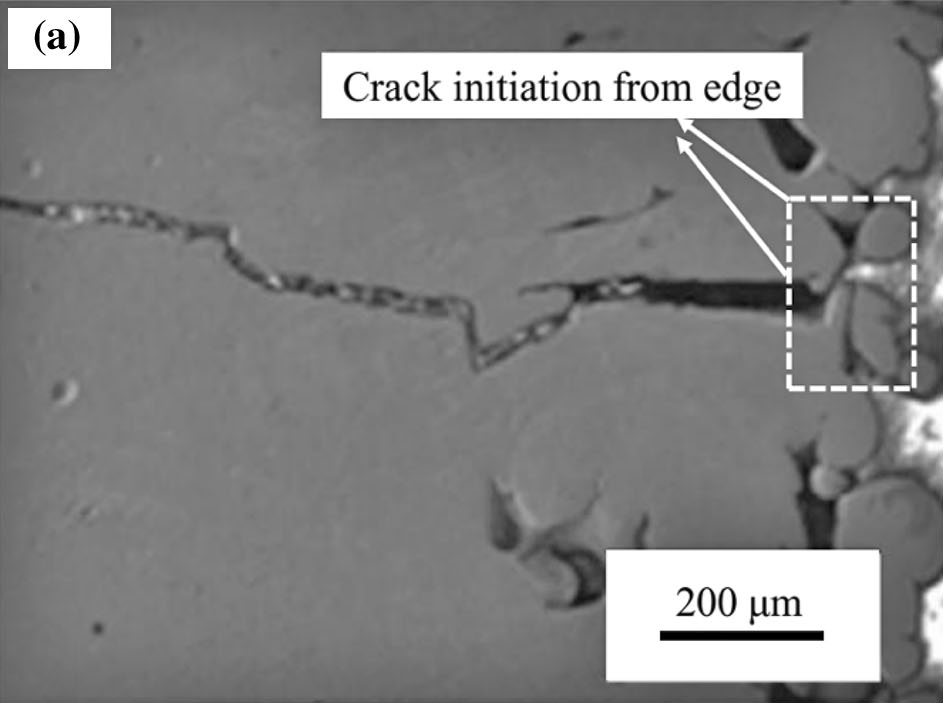
\includegraphics[width=0.885\textwidth]{theory/img/defects/cracks_part.png}
			\caption{Crack starting from surface propagating into the material \cite{zhang2017defect}}
		\end{figure}
		}
	\end{column}
\end{columns}
\end{frame}

\begin{frame}{Defects in SLM - Lack of fusion (LOF)}
\begin{columns}
	\begin{column}{0.5\textwidth}
		\visible<2->{
		\begin{figure}
			\centering
			\captionsetup{justification=centering}
			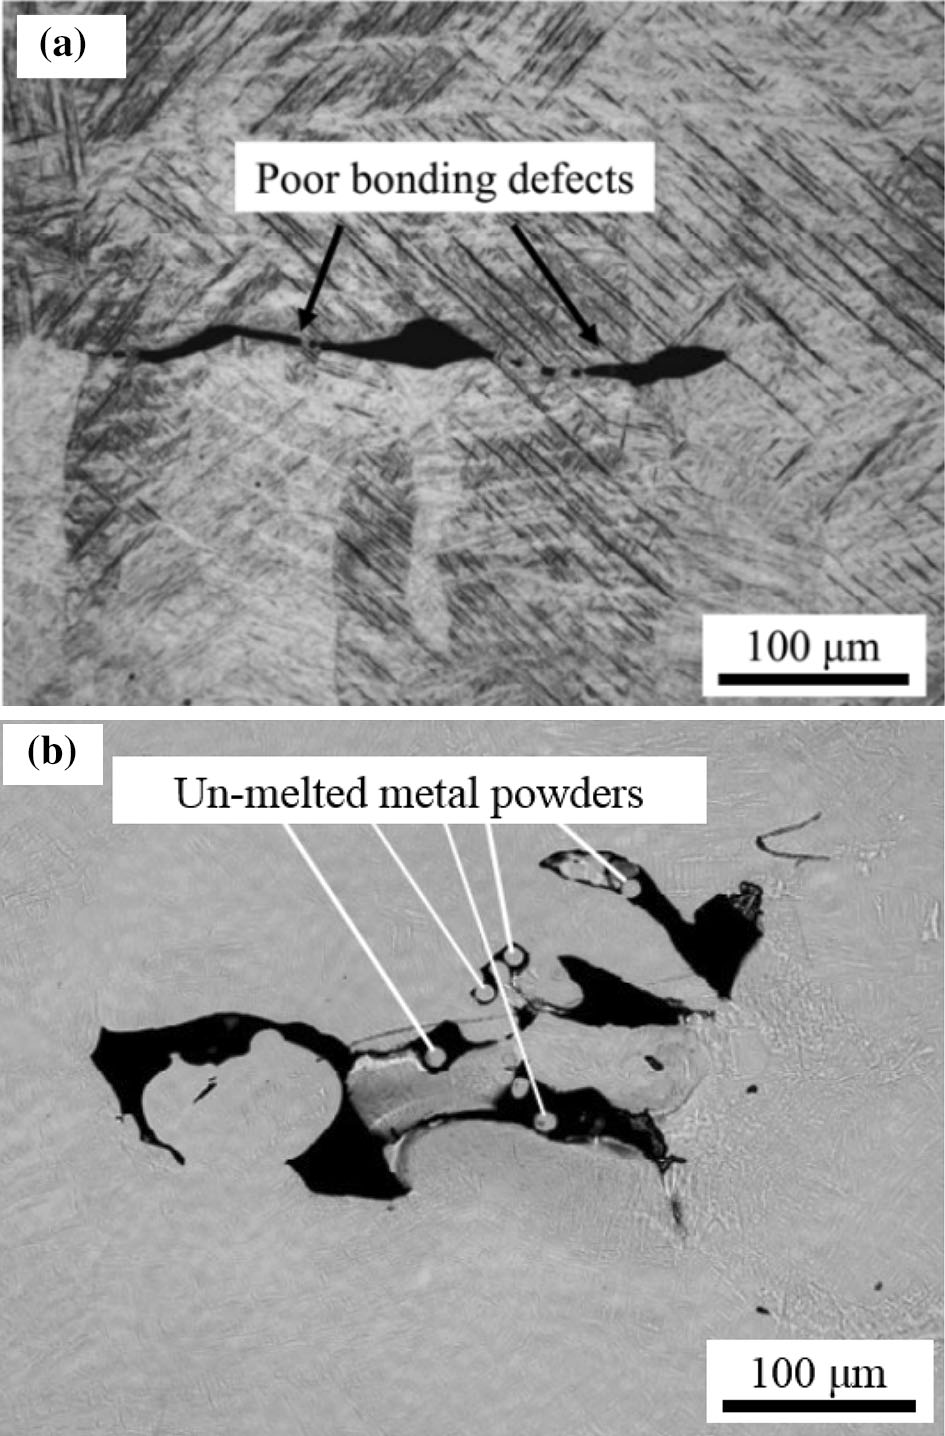
\includegraphics[trim=0 730 0 0, clip, width=0.9\textwidth]{theory/img/defects/lack_of_fusion.png}
			\caption{Lack of fusion of two traces due to insufficient overlap \cite{zhang2017defect}.}
		\end{figure}
		}
	\end{column}
	\begin{column}{0.5\textwidth}
		\visible<3->{
		\begin{figure}
			\centering
			\captionsetup{justification=centering}
			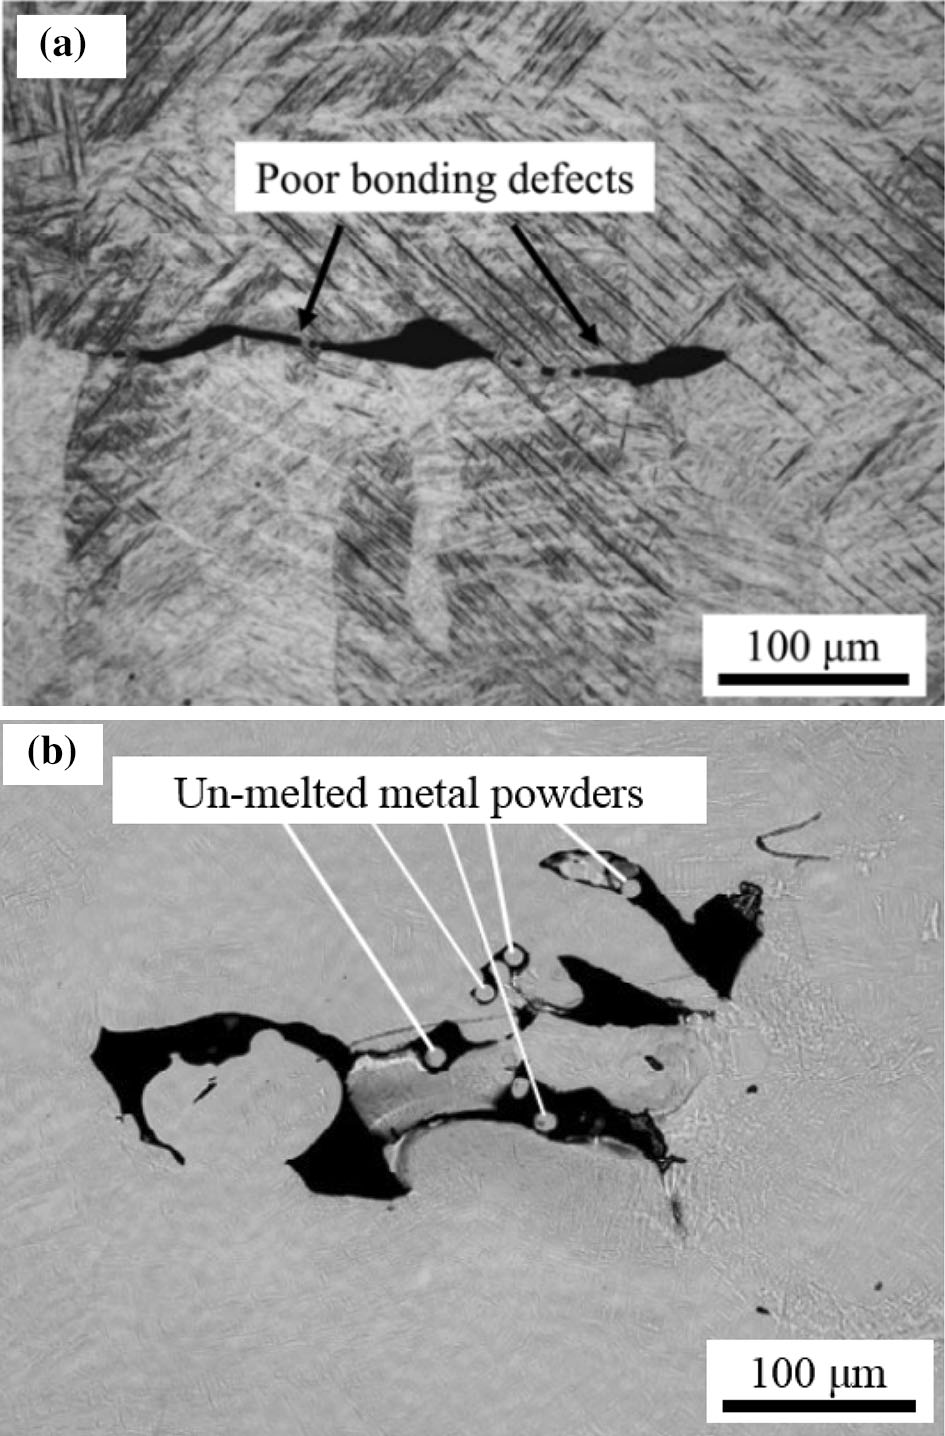
\includegraphics[trim=0 5 0 720, clip, width=0.9\textwidth]{theory/img/defects/lack_of_fusion.png}
			\caption{Lack of fusion resulting in unmelted powder included in voids \cite{zhang2017defect}.}
		\end{figure}
		}
	\end{column}
\end{columns}
\end{frame}


\begin{frame}{Defects in SLM - Keyhole effect}
	\visible<2->{
	\begin{figure}
		\centering
		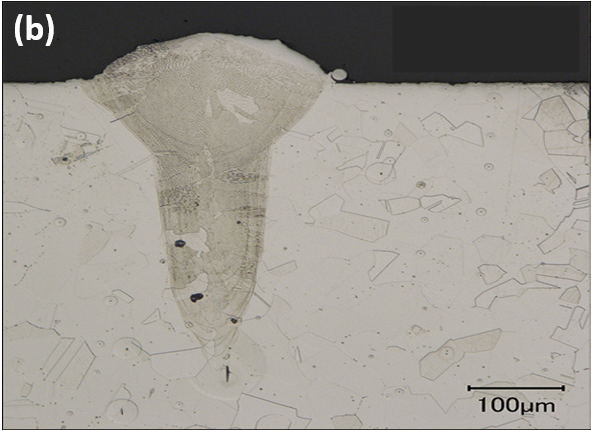
\includegraphics[width=0.5\textwidth]{theory/img/defects/keyhole.png}
		\caption{Defect due to occurence of keyhole effect \cite{eskandarisabzi2019defect}.}
	\end{figure}
	}
\end{frame}


\begin{frame}{Parameters}
\begin{columns}
	\begin{column}{0.5\textwidth}
		\begin{itemize}[<+->]
			\item Result influenced by choice of parameters
			\item High influence:
			\begin{itemize}
				\item scanning speed
				\item hatch distance
				\item layer thickness
				\item laser power
				\item spot size
			\end{itemize}
			\vspace{1cm}
			\item[$\Rightarrow$] Non-linear behavior\\
			Interplay is significant
		\end{itemize}
	\end{column}
	\begin{column}{0.5\textwidth}
		\visible<2->{
		\begin{figure}
			\centering
			\captionsetup{justification=centering}
			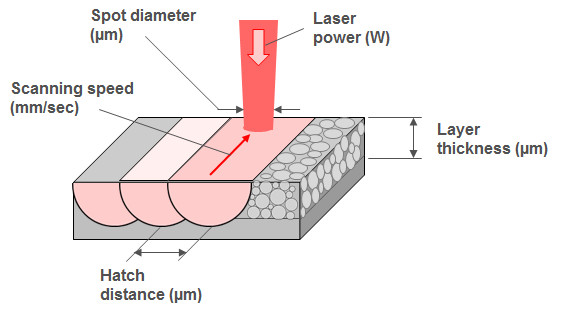
\includegraphics[width=\textwidth]{theory/img/slm_parameters.jpg}
			\caption{Most important parameters relevant to SLM \cite{saunders2017x}.}
		\end{figure}
		}
	\end{column}
\end{columns}
\end{frame}


\subsection[Modelling SLM with MD]{Modelling selective laser melting with molecular dynamics}
\begin{frame}{Molecular dynamics (MD) - Basic idea}
	\begin{itemize}[<+->]
		\item Atomistic approach of modelling many-body systems
		\item Individual trajetories by solving Newton's equations of motion explicitly:
		\begin{align}
			m_i \ddot{\uvec{x}}_i &= \uvec{F}_i
		\end{align}
		with the force $\uvec{F}_i$ being
		\begin{align}
			\uvec{F}_{i} &= \sum_{\substack{j=0\\j \neq i}}^{N-1} \uvec{F}_{ij}
			= -\sum_{\substack{j=0\\j \neq i}}^{N-1} \nabla_i U_j = -\nabla_i U
		\end{align}
		\vspace{0cm}
		\item[$\Rightarrow$] Problem: no analytical solution for $N \geq 3$
	\end{itemize}
\end{frame}


\begin{frame}{Molecular dynamics (MD) - LJ Potential}
\begin{columns}
	\begin{column}{0.55\textwidth}
		\begin{itemize}[<+->]
			\item Weak but long-range Van-der-Waals interactions
			\begin{align}
				\text{London dispersion force:} && F &\sim r^{-6}
			\end{align}
			\item Strong but short range Pauli exclusion $\sim r^{-12}$
			\item[$\Rightarrow$] Lennard-Jones potential (LJ)
			\begin{align}
				U^\text{LJ}(r) &= 4\epsilon \left[
					\left(\frac{\sigma}{r}\right)^{12}
					-
					\left(\frac{\sigma}{r}\right)^{6}
				\right] \\[10pt]
				\uvec{F}_{ij}^\text{LJ}(r) &= 24\epsilon \frac{\uvec{r}_{ij}}{r^2} \left[
					2\left(\frac{\sigma}{r}\right)^{12}
					-
					\left(\frac{\sigma}{r}\right)^{6}
				\right]
			\end{align}
		\end{itemize}
	\end{column}
	\begin{column}{0.4\textwidth}
		\visible<3->{
		\begin{figure}
			\centering
			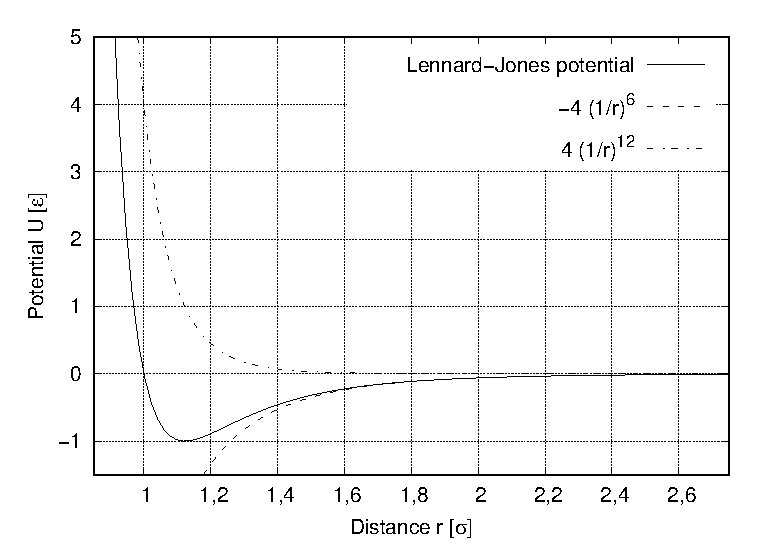
\includegraphics[width=\textwidth]{theory/plt/lennard_jones_en.eps}
			\caption{Lennard-Jones potential in units of $\sigma$ and $\epsilon$}
		\end{figure}
		}
	\end{column}
\end{columns}
\end{frame}


\begin{frame}{Molecular dynamics (MD) - Summarized}
\begin{columns}
	\begin{column}{0.7\textwidth}
		\begin{center}
			\color{gray}
			$\displaystyle m_i \ddot{\uvec{x}}_i = \sum_{j \neq i} \uvec{F}_{ij} $
		\end{center}
		\begin{itemize}
			\item<2->[] Iterative approach:
			\begin{tikzpicture}
				\draw[white] (0,0) -- (0,0.5);
				\node (forces) [flowchart, minimum width=0.8\textwidth, visible on=<3->] at (0,0) {Calculate $\{\uvec{F}_{ij}\}$ at $t$};
				\node (newton) [flowchart, minimum width=0.8\textwidth, visible on=<4->] at (0,-1.1) {Solve Newton's equations};
				\node (phasespace) [flowchart, minimum width=0.8\textwidth, visible on=<5->] at (0,-2.2) {Phase space coordinates $\{\uvec{x}_i\}$ and $\{\uvec{p}_i\}$ at $t+\Delta t$};
				\draw [arrow, visible on=<4->] (forces) -- (newton);
				\draw [arrow, visible on=<5->] (newton) -- (phasespace);
				\draw [arrow, visible on=<6->] (phasespace) -- (-5.2, -2.2) -- (-5.2, 0) -- (forces);
				%\draw [brown] (current bounding box.south west) rectangle (current bounding box.north east);
			\end{tikzpicture}
		\end{itemize}
	\end{column}
	\begin{column}{0.3\textwidth}
		\visible<3->{
		\begin{figure}
			\centering
			\visible<3->{
			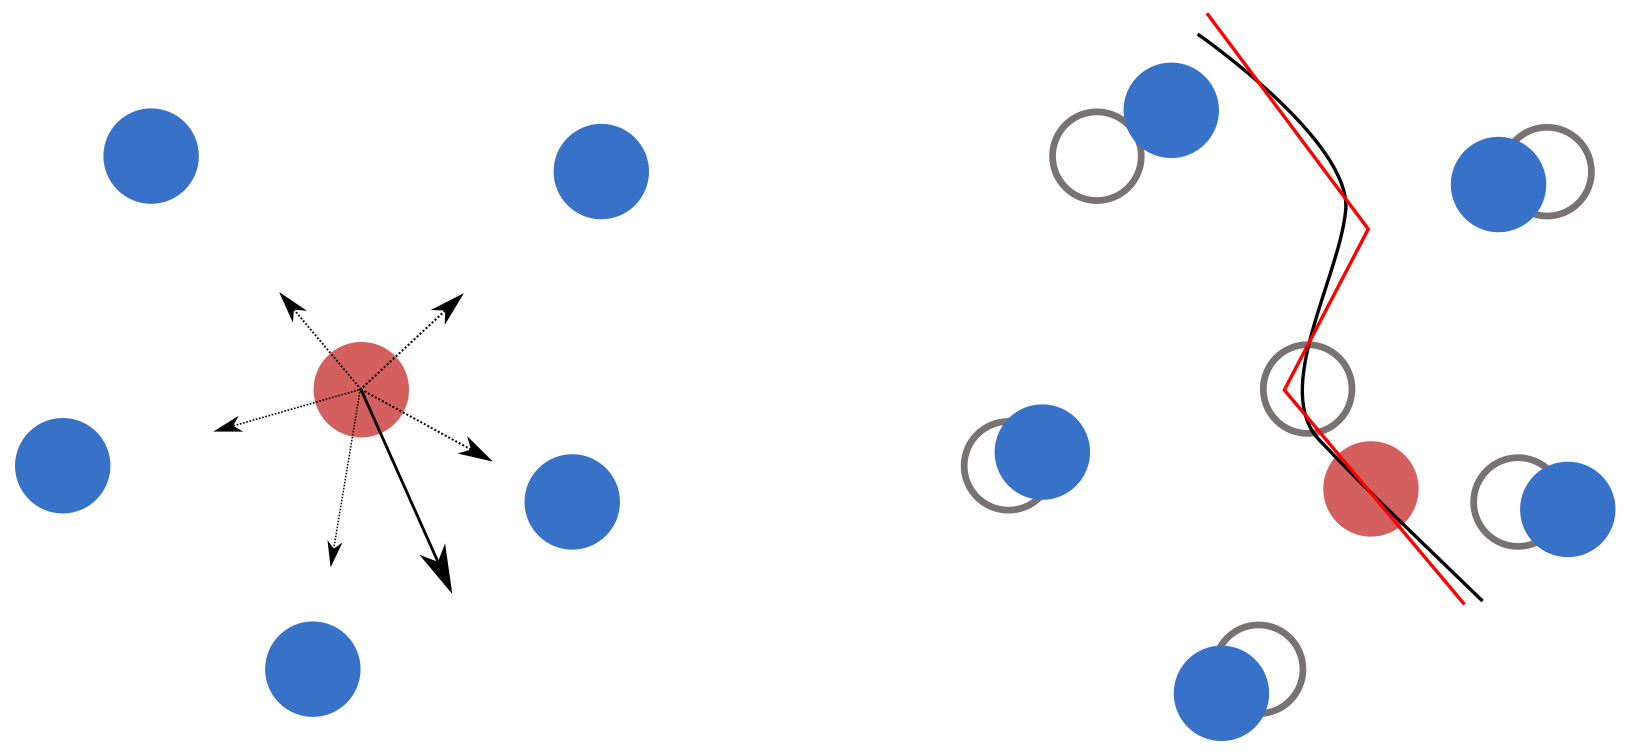
\includegraphics[trim=0 70 950 100, clip, width=0.6\textwidth]{theory/img/scheme_md.png}
			}
			\visible<5->{
			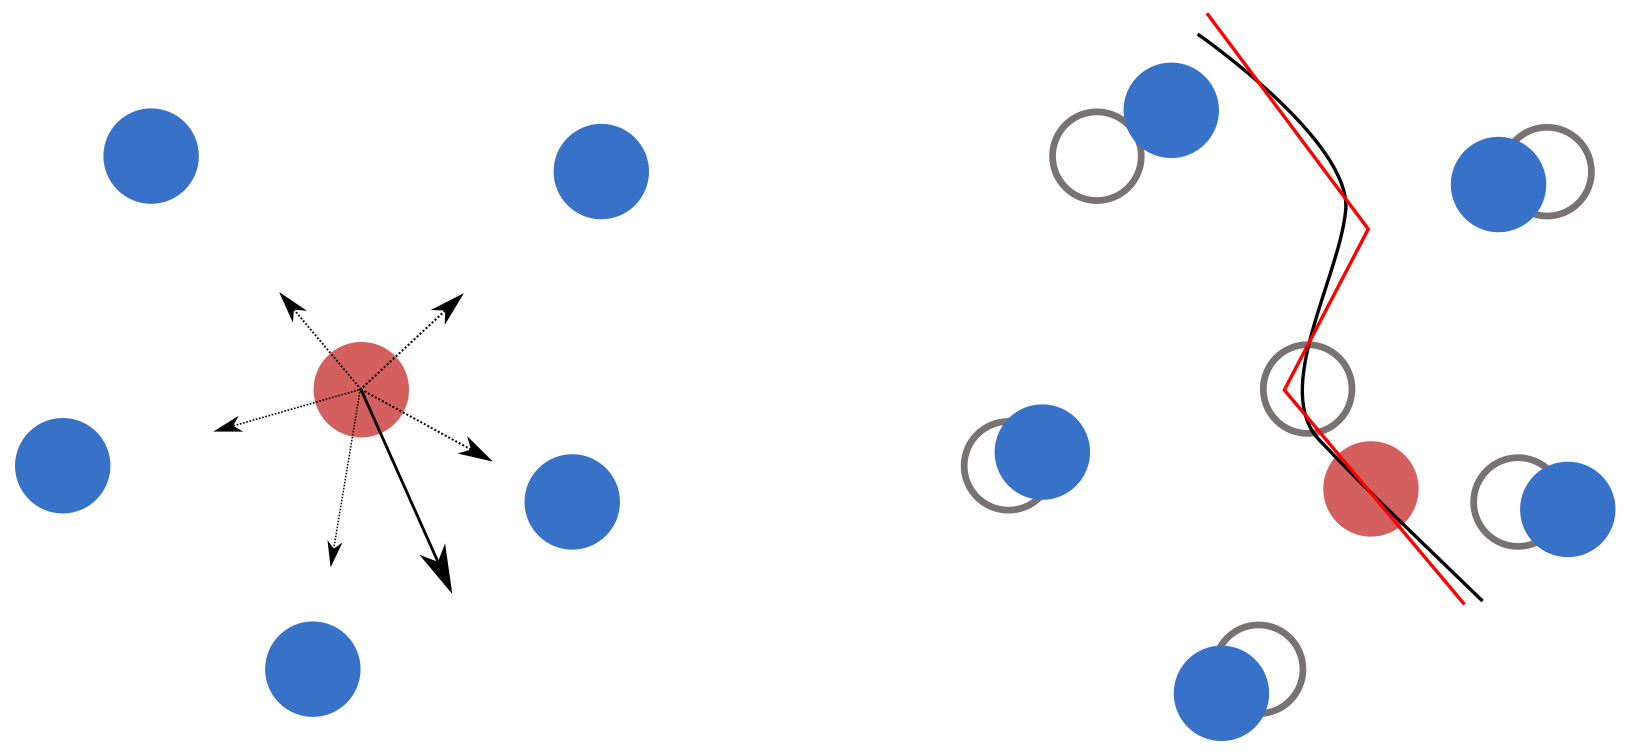
\includegraphics[trim=950 50 0 -50, clip, width=0.6\textwidth]{theory/img/scheme_md.png}
			}
			\caption{Basic principle behind MD \cite{sonntag2011computer}.}
		\end{figure}
		}
	\end{column}
\end{columns}
\end{frame}


\begin{frame}{Implementation of the laser}
	\begin{itemize}[<+->]
		\item $T$ and $E_\text{kin}$ connected through equipartition theorem
		$\left\langle E_\text{kin} \right\rangle = \frac{f}{2} k_\text{B} T$
		\item[$\Rightarrow$] Velocity rescaling with factor
		$a = \sqrt{1+  {\color{red} \dx[E]} / E_\text{kin}(t)}$
		\item Gaussian laser intensity profile: $I(x,y) = \frac{P_\text{tot}}{2\pi \sigma^2} \exp\left( -\frac{x^2+y^2}{2\sigma^2} \right)$
		\item[] + Absorption with Lambert-Beer's law: $I(x,y,z) = I(x,y) \cdot \exp\left(-\mu z\right) {\color{gray} \cdot (1-R)}$
		\vspace{0.5cm}
		\item Local intensity: $\dx[I] = \dfrac{\dx[E]}{\dx[A] \cdot \dx[t]}$
		\item[$\Rightarrow$]
		\begin{align}
			\dx[E] = \frac{\dx[I]}{\color{gray} \dx[z]} \cdot {\color{gray} \dx[z]} \cdot \dx[A] \cdot \dx[t]
				= (1-R) \cdot \mu \cdot \exp\left(-\mu z\right)
				\cdot \frac{P_\text{Ges}}{2\pi \sigma^2}
				\cdot \exp\left(-\frac{x^2 + y^2}{2\sigma^2}\right)
				\cdot \dx[V] \cdot \dt
		\end{align}
	\end{itemize}
\end{frame}
